
\chapter{Requirements} 
{\setstretch{1.85}

\section{Introduction}
This chapter will explore the requirements of the final system. In this project I am being assisted by Dr. Alasdair J G Gray, an Associate Professor in Computer Science at Heriot-Watt University. Dr. Gray leads the Bioschemas community, meaning he can provide detailed requirements of what the system should be able to provide, additionally providing feedback as a user and encouraging the community to try the tool. \par

In this chapter, I will give an overview of the systems desired functionality, discuss the requirements gathered from Bioschemas as well as my initial prototype systems and how they aided in establishing the final system requirements. Finally, a MoSCoW analysis of the system requirements will be completed. 

\section{System Requirements}
\subsection{Overview}
Once the system is complete it should allow the user to select a Bioschemas profile that they would like to generate a markup for. A form should then appear allowing the user to enter the data required to create the markup for the selected profile. The system then provides the user with all the information they need to complete the form without having to go to any external sources or read any documentation. Once complete, the system then generates the markup with the provided data. The user will then be able to validate the generated markup is correct, both syntactically and against the profile.

}

\subsection{Bioschemas}
\label{sec:bioschemaRequirements}
As mentioned in Section \ref{sec:bioschema}, Bioschemas adds not only new biological types to Schema.org but also a profile layer over the Schema.org model with additional constraints. To support Bioschemas profiles, the system must be able to support these additional constraints: cardinality (one or many items for a specified property), marginality (Minimum, Recommended and Optional properties) and use of controlled vocabularies. 

Through discussions with Dr. Gray, I was able to establish that the system should use a declarative description of the Bioschemas profiles in order to generate the form. The form should also be ordered in a way that makes most sense to the user. i.e Minimum then Recommended then Optional properties. Additionally, the generated markup should be in the format of JSON-LD (See Section \ref{sec:jsonld}).

Finally, the system should display all the information required for the user to fill out the form. Where the information is available, each property should provide a description, examples and controlled vocabularies, which are provided by Bioschemas and Schema.org.

\subsection{Prototyping}\label{ch:prototyping}
To gain a better understanding of the system and its requirements I developed a prototype system. The goal of the prototype was to create a form that allowed users to generate a markup for the Dataset (v0.2)\footnote{\url{http://bioschemas.org/specifications/Dataset/} (accessed 03/11/2018)} Bioschemas profile. Through developing the prototype one functional requirement was discovered and another's importance was highlighted.

During development I discovered that in order to generate markup based on the Bioschemas Dataset (v0.2) profile, the form must be able to handle recursive property types. This is due to Schema.org types having the ability to contain themselves as an expected type for a property. For example, the Schema.org type PropertyValue\footnote{\url{https://schema.org/PropertyValue} (accessed 03/11/2018)} has a property valueReference, where the expected type for this property can either be Enumeration, QualitativeValue, QuantiativeValue, StructuredValue or itself a PropertyValue. This requirement was then added to the list of functional requirements as FR 7 in Table \ref{table:2}. The requirement's prioritisation was set to should as unfortunately at this stage I was not able to produce this functionality, later discussed in Section \ref{sec:jsoneditor}.

\newpage
The requirement highlighted during prototype development was FR 5, the system must be able to handle cardinality and marginality, shown in Table \ref{table:2}. The cardinality portion of this requirement previously mentioned in Section \ref{sec:bioschemaRequirements}, was not possible during the first iteration of the prototype due to limited functionality with the library used to display the form, this limitation will be later discussed in Section \ref{sec:jsoneditor}.


Once the prototype system was complete, shown in Figure \ref{fig:bioProto}, a initial prototype usability evaluation was carried out to tailor the system requirements towards to the target user-group (members of the Bioschemas and life science communities). The feedback showed us that the functional requirements of the system achieved the desired functionality although more information needed to be provided thus FR 10 (Descriptions and Examples) and 11 Controlled Vocabulary) were added. Additionally, one test subject recommended to include different formats of markup and so FR 12 (Microdata and RDFa) was included. A more detailed discussion of the prototype usability evaluation and the results can be seen in Section \ref{sec:prototyUsability}.\newline

\begin{figure}[h]
 \centering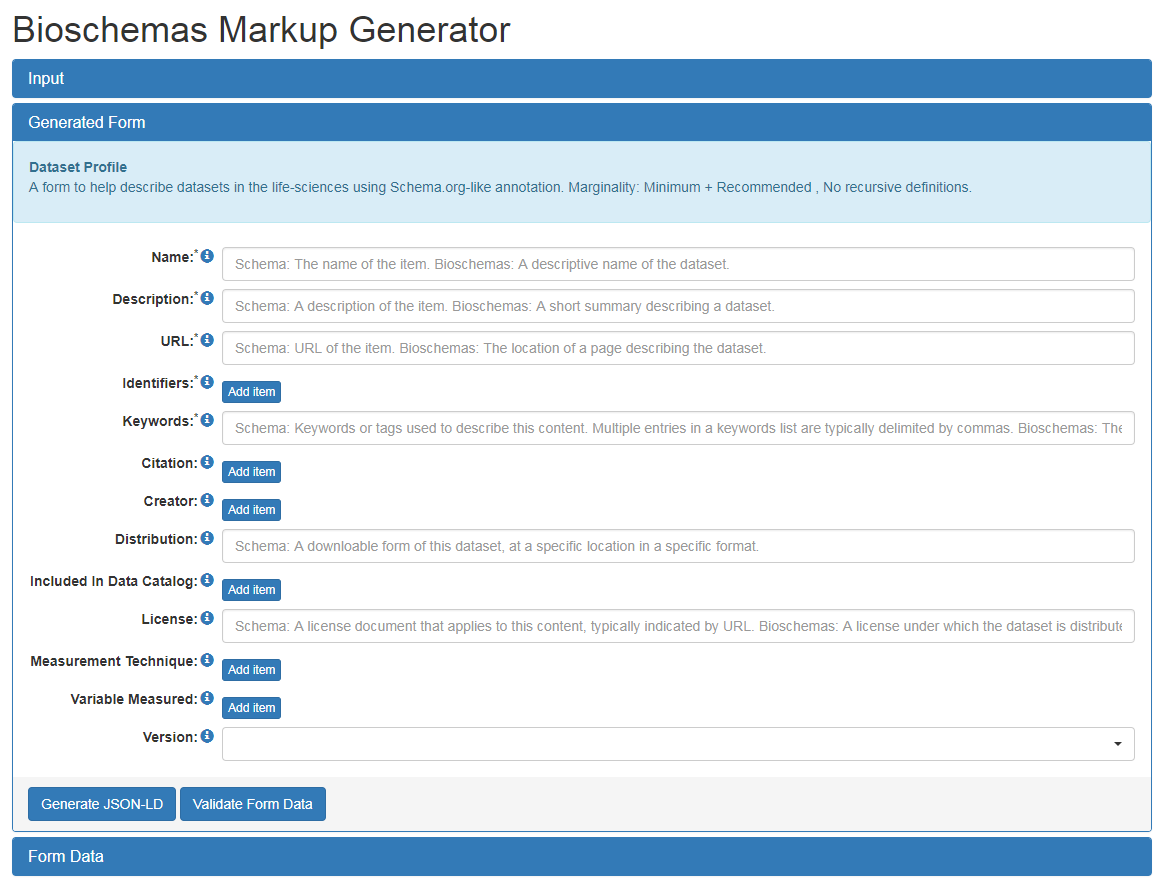
\includegraphics[scale=0.5]{images/bioschemasPrototype.PNG}
   \caption{Bioschemas Markup Generate Prototype Second Iteration}
   \label{fig:bioProto}
\end{figure}

\newpage
\section{MoSCoW Requirements Analysis}
From the requirements in Section \ref{sec:bioschemaRequirements} above along with any other requirements gathered, a MoSCoW analysis was performed on the requirements detailing the priority of each. The requirements have been split into two categories: Functional Requirements Table (\ref{table:2}) and Non-Functional Requirements Table (\ref{table:3}).

\subsection{Functional Requirements}\label{sec:functionalReq}
{\setstretch{1.2}

\begin{longtable}{ |p{1.5cm}|p{1.75cm}|p{5cm}|p{5cm}|  }
 \hline
 \multicolumn{4}{|c|}{Functional Requirements} \\
 \hline
 ID & Priority &Requirement& Reasoning\\
 \hline
 FR 1   & Must & The system must allow users to enter data into the form. & 
 This is core functionality of the system.\\
 \hline
 FR 2   & Must & The system must generate JSON-LD compliant data.&
 This is core functionality of the system.\\
  \hline
 FR 3   & Must & The system must allow users to select the Bioschemas profile.&  
 This allows users to be able to select the Bioschemas profile that they would like to generate the markup for.\\
  \hline
 FR 4  & Must & The system must be able to handle Schema.org data types\footnote{\url{https://schema.org/DataType} (accessed 03/11/2018)}.& 
 This is necessary to be able to support the user in entering the data types that Bioschemas allows.\\
   \hline
 FR 5   & Must & The system must be able to handle cardinality and marginality.&
 This is core functionality of the system to support BioSchemas profiles.\\
   \hline
  FR 6   & Should & The system should generate the forms based on a declarative specification.&
 This allows the system to be more dynamic and not be rely on static form definitions. Supporting the evolution of Bioschemas.\\
  \hline
 FR 7   & Should  & The system should be able to handle recursive properties.&
 This allows recursion that may occur in Schema.org properties.\\
   \hline
 FR 8   & Should  & The system should be able to prioritise form inputs.&
 The form should be ordered in a way that is intuitive for the user.\\
   \hline
 FR 9   & Should  & The system should be able validate the generated markup against the Bioschemas profile .&
 The user should be certain that the generated markup is correct.\\
    \hline
 FR 10   & Should  & The system should display a description of each property, as well as examples.&
 To allow users to get more information without going to external sources. \\
  \hline
  FR 11   & Should  & The system should display the controlled vocabulary of each property.&
 To allow users to see the controlled vocabulary to use without going to external sources. \\
  \hline
 FR 12  & Could    & The system could generate Microdata and RDFa along side JSON-LD.& 
 Allow users to have a choice of format generated.\\
  \hline
 FR 13  & Could    & The system could allow the user to download the data generated. & Allow users to easily save their results without having to use external software.\\
  \hline
 FR 14   & Wont    & The system wont be able to dynamically update declarative specifications from an online source. &
 To stop the systems functionality from going down if the declarative specification is incorrect. \\
 \hline
 \caption{Table of Functional Requirements}
 \label{table:2}
\end{longtable}


\subsection{Non-Functional Requirements}

\begin{longtable}{ |p{1.5cm}|p{1.75cm}|p{5cm}|p{5cm}|}
 \hline
 \multicolumn{4}{|c|}{Non-Functional Requirements} \\
 \hline
 ID & Priority &Requirement& Reasoning\\
 \hline
 NFR 1   & Must &The system must be easy to use through a simple user interface.&
 A systems interface should be intuitive to use.\\
 \hline
 NFR 2   & Must &The system must be available 24/7 &
 The system should be available at all times to support potential users across the globe. \\
 \hline
 NFR 3   & Should &The system should be accessible through the top internet browsers: Google Chrome, Mozilla Firefox and Apple Safari. &
 To allow the most users access to the system.\\
 \hline
 NFR 4   & Could &The system could have two interfaces. One for standard users. Another for administrative users. &
 To allow more advanced users greater functionality to generate more complex markups.\\
 \hline
 \caption{Table of Non-Functional Requirements}
\label{table:3}
\end{longtable}

}